\documentclass[../Hovedrapport.tex]{subfiles}
\begin{document}

%---------------------------------------------------------------
% Der mangler følgende
% - Specifikation til program (Hvad end dette betyder)
% - Liste over måleinstrumenter (og usikkerheder)
%  - Flowchart over program

% Som der står:
%I M4PRJ’s rapport skal medtages specifikation til program, liste over måleinstrumenter inklusiv måleusikkerheder samt flowchart over program.
%---------------------------------------------------------------------
\chapter{Instrumentering}
    \label{sec:instrumentering}

For at gøre det muligt at sammenholde de forudbeskrevede beregningsmodeller med realdata fra prototypen, er det nødvendigt at tage målinger af temperaturer og tryk på systemet under drift. 
Der vil i følgende afsnit blive gennemgået henholdsvis installationsforhold for de forskellige komponenter, hvor de forskellige komponenter er placeret samt, hvordan de forskellige komponenter bliver kalibreret. Alt dette foretages med henblik på at validere forsøg såvel som udregninger. Målinger af tryk og temperaturer er foretaget med en software udviklet i \textit{NI LabVIEW 18}. Programmet er udarbejdet i forbindelse med semesterprojektet, hvortil der er opsat forskellige krav til programmet, som er analyseret ved \textit{MoSCoW Metoden}. Kravspecifikationen for det endelige program fremgår af appendiks \ref{sec:specs_p24}.
%---------------------------------------------------------------------
\section{Installationsforhold (M.N. \& U.H.)}   
I forsøgene vil de fleste af målingerne blive foretaget med \textit{National Instruments} myDAQ og cDAQ. Disse apparater måler små spændingsforskelle ved eksempelvis thermocouples, som bliver transformeret til digital data. Dette betyder, at de er letpåvirkelige over for indflydelse fra de ydre omgivelser. Denne ydre påvirkning kaldes støj, og netop denne kan tilnærmelsesvis undgås ved korrekt jording og gennemtænkt ledningsføring. Tryktransmitterne er eksempelvis jordet for at undgå denne støj. Foruden jording, er gennemtænkt ledningsføring også et punkt, som kan sikre valide måleresultater, hvilket bl.a. gøres ved, at strømførende ledninger, der skal passere sensorledninger, krydser hinanden med 90\si{\degree} imellem. Desuden kan det være en god idé at bruge skærmede kabler, så disse har så lidt indflydelse på måleresultaterne som muligt. 
%---------------------------------------------------------------------
\section{Sensorer (M.N. \& U.H.)}
Der er en række forskellige sensorer på prototypeanlægget, som skal måle de forskellige værdier af henholdsvis tryk, temperatur og el-effekten. Disse sensorer er essentielle for forsøgene, hvorfor de er placeret i interessepunkter. Placeringen af trykmålerne er før og efter kompressoren, hvortil thermocouples placering fremgår af figur \ref{fig:placthermo}.
\begin{figure}[H]
	\centering
	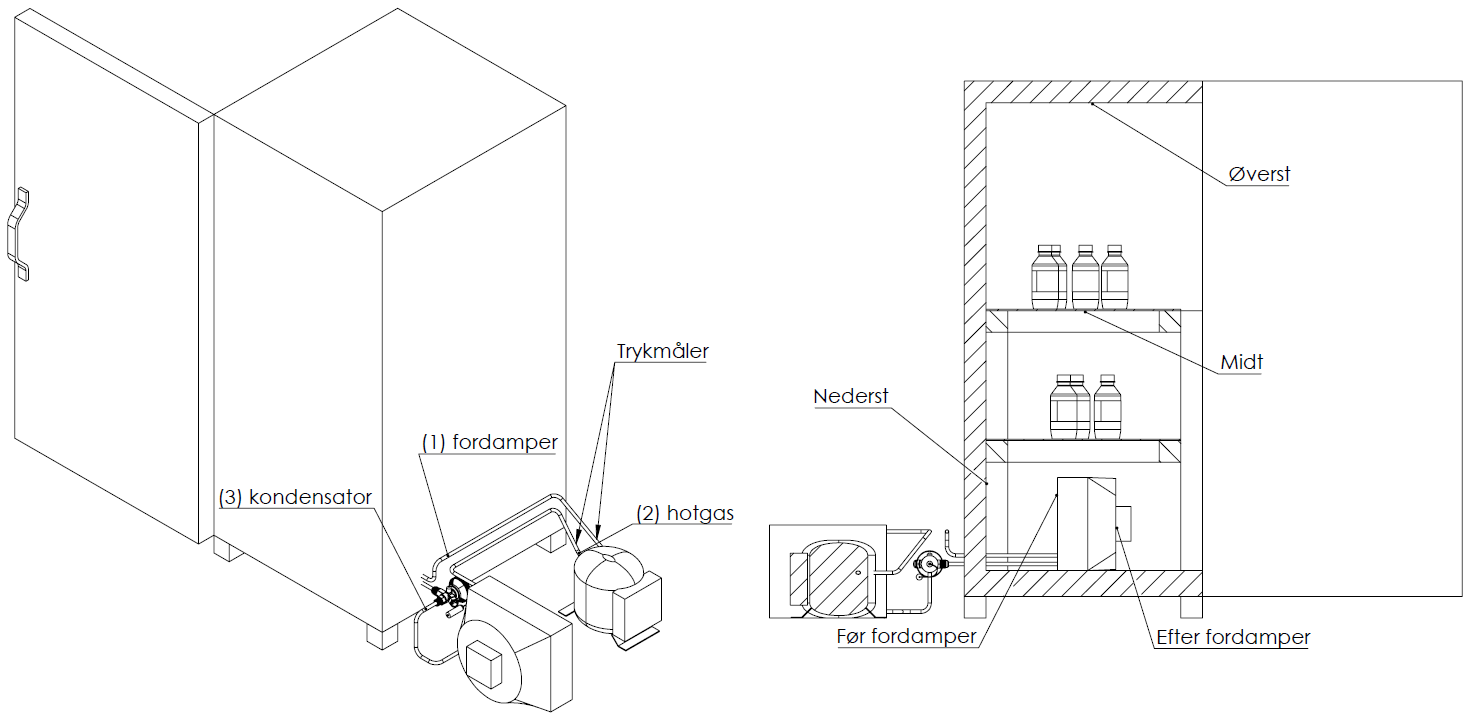
\includegraphics[width=1\textwidth]{Billeder/maalerplacering.png}
	\caption{\textit{Placering af thermocouples og trykmålere}.}
	\label{fig:placthermo}
\end{figure}

\subsection{Temperaturmålinger (B.B. \& N.J.)}
Selve temperaturmålingerne bliver foretaget med thermocouples, hvor disse måler spændingsforskellen mellem to metaltråde. Thermocouples består af to metaltråde, hvor enderne på de to metaltråde er sat sammen. Det er i denne ende, hvor temperaturerne bliver målt. De to ender, som ikke er sat sammen, indsættes i eksempelvis en cDAQ, hvor spændingforskellen bliver målt og omsat til en temperatur. Spændingen, der måles og omsættes til en temperatur, bestemmes ud fra følgende formel:
\begin{align}
    e=a_1\cdot T+a_2\cdot T^2+a_3 \cdot T^3+...a_n\cdot T^n
\end{align}
I ovenstående ligning er $a_1,a_2...a_n$ kalibreringskonstanter for sensoren med enheden $\dfrac{V}{K^n}$, og $T$ er den målte temperatur.

I forsøget bliver der anvendt thermocouples af typen J, og disse har en præcision på $\pm 0,75\%$. Disse thermocouples har et måleinterval på mellem \SI{-200}{\celsius} og \SI{+1300}{\celsius}. 

Der er i alt anvendt ti thermocouples til at måle forskellige interessepunkter på køleanlægget. På selve anlægget er der påsat et thermocouple efter fordamperen, før ventilen og et til at måle hotgastemperaturen. Der sidder desuden tre thermocouples fordelt rundt i køleskabet. Disse thermocouples er placeret således, at et befinder sig i toppen af køleskabet, et i midten og det sidste er placeret i bunden af køleskabet. Disse thermocouples er placeret et stykke væk fra køleskabsvæggen, hvilket vil give et mere korrekt billede af lufttemperaturen i køleskabet, da vægtemperaturen herved vil influere i mindre grad. Slutteligt er der fire frie thermocouples, som frit kan manøvreres rundt i køleskabet til eksempelvis måling af temperaturen på væsken i indsatte flasker.
%---------------------------------------------------------------------
\subsection{Trykmåling (J.K. \& C.R.)}
Der er i kølekredsen blevet monteret to trykmålere af typen \textit{Danfoss AKS 32}. Der er en højtryks- og lavtrykside, hvor disse trykmålinger bliver foretaget. Lavtrykssiden er placeret lige inden kompressoren og efter fordamperen, mens højtrykssiden er placeret lige efter kompressoren og inden kondensatoren. Den maksimale temperatur, hvorved tryktransmitteren kan operere, afhænger af omgivelsestemperaturen, som i dette tilfælde er antaget til at være \SI{30}{\celsius}. Ud fra følgende ligning kan maksimaltemperaturen på fluiden bestemmes:
\begin{align}
t_{max}=115-(0,35\cdot t_{opr})=104,5\si{\celsius}
\end{align}
 Ud fra procesværdierne i tabel \ref{tab:procesval_med_h2} fremgår det, at ingen af temperaturværdierne overskrider denne temperatur. Desuden fremgår det af databladet for tryktransmitteren, at den har en nøjagtighed på $\pm 0,8 (max.)$ og en $\pm0,3 (nom.)$ inklusiv ikke-linearitet, hysterese og repeterbarhed \ref{sec:bil_tryk}. 
%---------------------------------------------------------------------
\section{Kalibrering}
For at opnå valid data er det vigtigt, at måleinstrumenterne er kalibreret korrekt. Der er sjældent store forskelle på kalibreringsmetoderne for diverse komponenter. Dog kræver en succesfuld kalibrering et kendskab til et veldokumenteret referencepunkt. Dette referencepunkt kan eksempelvis være frysepunktet for vand ved $0\si{\celsius}$ for et thermocouple. Generelt er der ved kalibrering to hovedkomponenter; henholdsvis en DUT (Device Under Test) og en REF (Reference Device). DUT'en er den komponent, der ønskes kalibreret, mens REF'en er den allerede kalibrerede komponent, hvor usikkerheden på komponenten allerede kendes. Det er her vigtigt, at REF'en har en mindre usikkerhed end DUT'en, da det naturligvis ikke er acceptabelt at kalibrere komponenter, hvor referencepunktet har en større usikkerhed. Kalibreringen skal foretages over hele det område, der ønskes afdækket. 
%---------------------------------------------------------------------
\subsection{Kalibrering af tryksensor  (J.K. \& C.R.)}
Da tryktransmitterne er påsat systemet, og køleanlægget allerede er påfyldt kølevæske, har det ikke været muligt at foretage en optimal kalibrering af disse.
Under optimale omstændigheder ville tryktransmitterne være påsat systemet, men uden kølevæske. Derefter ville systemet blive påtrykt et referencetryk af et eksternt system, der kan hæve eller sænke trykket.
Eftersom dette ikke har været muligt, er trykmålerne blevet kalibreret op imod hinanden. 
For alligevel at kalibrere tryksensorerne har systemet været slukket i et par dage, således trykket på lav og højtrykssiden er udlignet. Dernæst kan trykket aflæses på de to tryktransmittere, hvor gennemsnittet af disse to er det, som antages at være referencetrykket i den pågældende situation. Dette betyder, at hvis der er en forskel på \SI{0,1}{bar} imellem de to sensorer, vil den ene sensor have en fejl på \SI{-0,05}{bar}, mens den anden har en fejl på \SI{0,05}{bar}. 
Dette er selvfølgelig ikke optimalt, men må anses for at være den bedste metode situationen taget i betragtning. 

Selve kalibreringsprogrammet er lavet i \textit{NI LabVIEW 18}, og funktionen af dette kan ses nedenfor:
\begin{figure}[H]
    \centering
    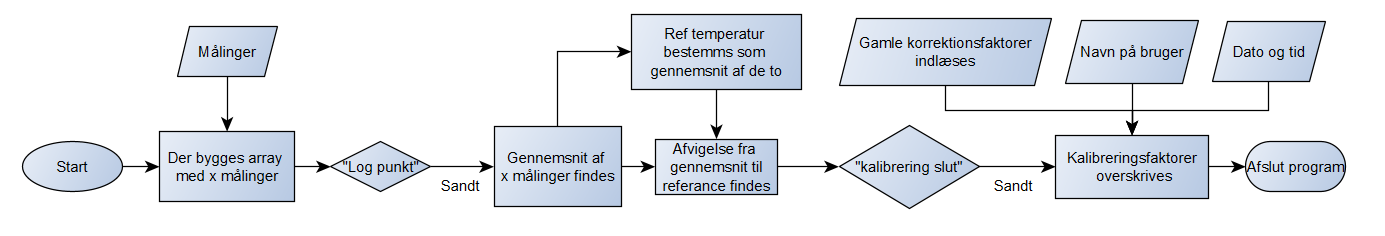
\includegraphics[width=1.0\textwidth]{Billeder/kali_tryk.png}
    \caption{\textit{Flowchart for trykkalibrering}}
    \label{fig:fc_tryk_kali}
\end{figure}
%---------------------------------------------------------------------
\subsection{Kalibrering af thermocouples (B.B. \& N.J.)}
For at kalibrere thermocouples er der også lavet et \textit{NI LabVIEW 18} program. Programmet har til formål at bestemme temperaturmålernes afvigelse, som funktion af temperaturen.
Funktionen af dette program kan ses afbildet i nedenstående figur.
\begin{figure}[H]
\centering
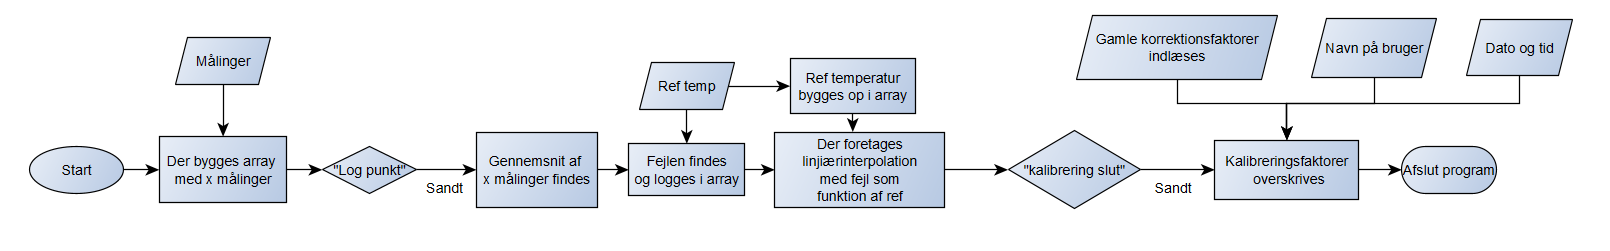
\includegraphics[width=1.0\textwidth]{Billeder/kai_thermo.png}
\caption{\textit{Flowchart for temperaturkalibrering}}
\label{fig:fc_tryk_kali}
\end{figure}

Til kalibrering af thermocouples bruges tørblokskalibratoren ITC155A. 

Her findes gennemsnittet af 51 målinger pr. referencetemperatur. Det er dette gennemsnit, som holdes op imod tørblokskalibratoren for at finde afvigelsen.
Der er målt i intervallet: -20, -10, 0, 10, 20, 30, 40, 50, 60 og 70 \si{\celsius}.
%---------------------------------------------------------------------
\section{Usikkerheder for thermocouples og tryktransmittere i anlægget (B.B. \& M.N.)}
    \label{sec:tryk_temp_usikkerheder}
Kalibreringen og korrigeringen for fejlen ved tryktransmitterne og thermocouples er benyttet til at opstille et valideret usikkerhedsbudget for disse sensorer til beregning af en samlet propageret usikkerhed. Dette er foretaget i henhold til \textit{GUM Metoden} (Propagation of uncertainty). GUM Metoden er en numerisk variansmetode til beregning af den propagerede usikkerhed, hvor der tages forbehold for de enkelte usikkerhedsbidrags fordelingstyper. Et valideret usikkerhedsbudget, hvor installationsforholdenes usikkerhed for thermocouples og tryktransmittere er taget i betragtning, er opstillet og fremgår af appendiks \ref{sec:ubudget_temp} og \ref{sec:ubudget_tryk}. De progaperede usikkerheder herfra fremgår af følgende tabel \ref{tab:tryk_temp_usikkerheder}:
\begin{table}[H] 
\centering
\begin{tabular}{|c|c|}  \rowcolor[gray]{0.7}                                            \hline
\multicolumn{2}{|c|}{\textbf{Usikkerhed af målesensorer i køleskabsanlægget}}       \\  \hline \rowcolor[gray]{.8}
\textbf{Betegnelse}         & \textbf{Værdi}                                        \\  \hline 
Trykusikkerhed              & $ \pm \SI{0,068}{\bar} $                            \\ \hline
Temperaturusikkerhed        & $ \pm \SI{1,398}{\celsius} $                       \\ \hline
\end{tabular} 
\caption{\textit{Usikkerhederne for tryk- og temperatursensorer}} 
\label{tab:tryk_temp_usikkerheder} 
\vspace{-20pt}
\end{table}
Disse usikkerheder er beregnet ved en k-faktor på $k=2$ og et konfidensniveau på $95\%$.    
\end{document}